\subsubsection{High-Level Component View}
\begin{figure}[!h]
\centering
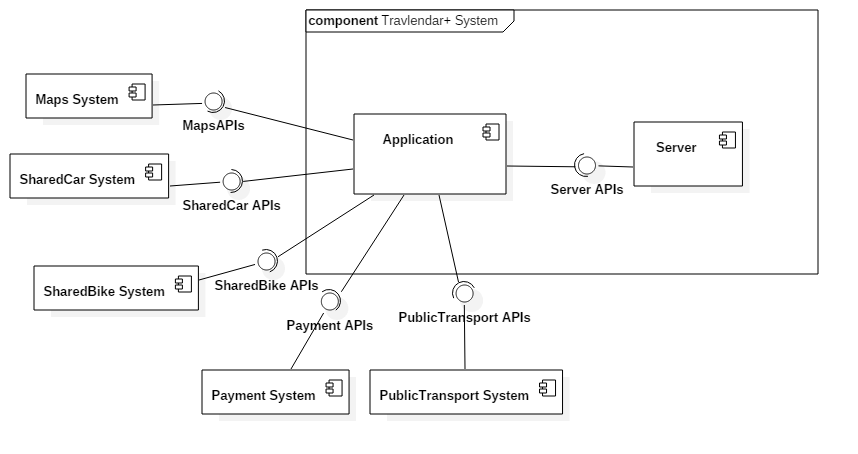
\includegraphics[scale=0.4]{images/ComponentDiagramSystem}
\caption{High Level Component View}
\label{ref:highlevelcomponentview}
\end{figure}
Component to be developed:
\begin{itemize}
\item
\textbf{Application:} It is the core of the system, it manages all information provided by the others services and performs the majority of the functions. It provides the client access to the entire system.
\item
\textbf{Server:} This component has an account manager and backup roles. It receives the data from the application and provides them when necessary (e.g. during the login operation).
\end{itemize}
Component to be integrated in the system:
\begin{itemize}
\item
\textbf{MapsSystem:} It is the provider of the maps and all necessary information for the computation of the journey.
\item
\textbf{SharedCarSystem, SharedBikeSystem:} Those component provide all information (availability, location and costs) respectively shared cars and shared bikes.
\item
\textbf{PublicTransportSystem:} It provides all information about the public transport of the city.
\item
\textbf{WeatherSystem:} It provides the weather forecasts in the city.
\item
\textbf{PaymentSystem:} This component provides the payment service.
\end{itemize}

\clearpage
\subsubsection{Application System}
\begin{figure}[!h]
\centering
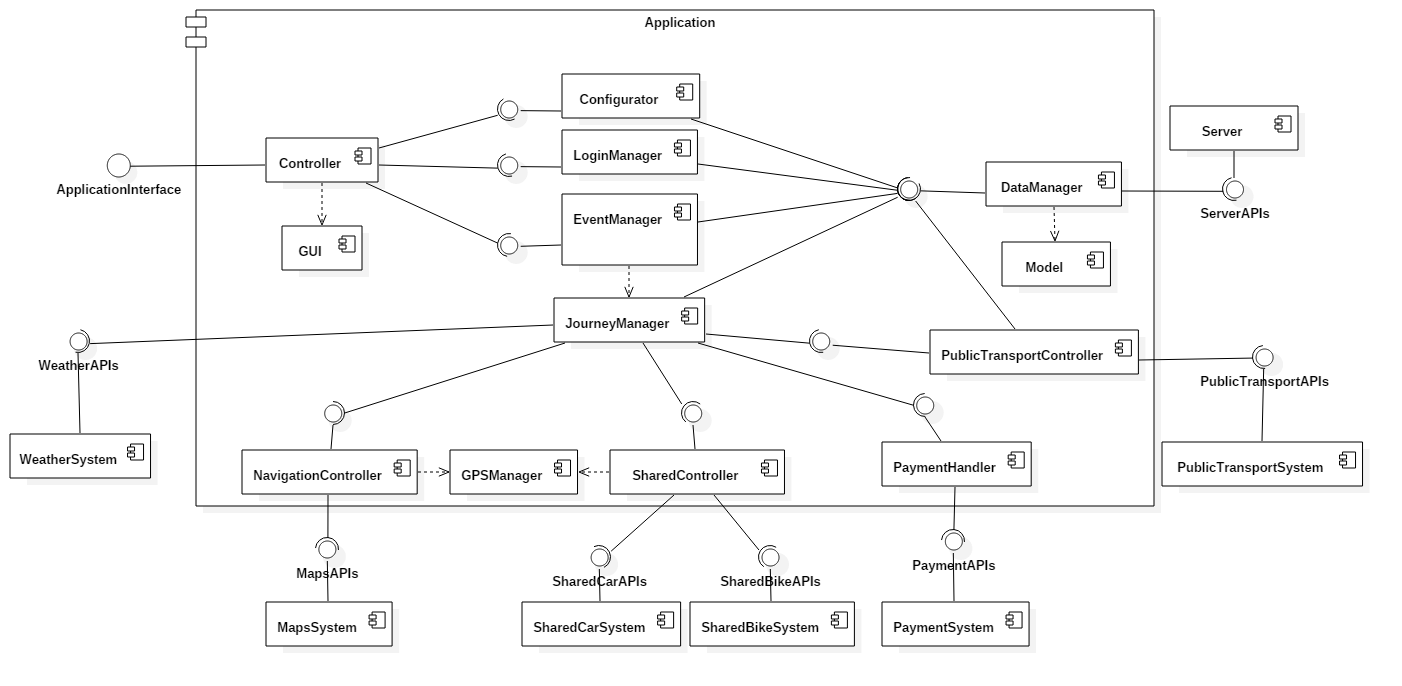
\includegraphics[scale=0.35]{images/ComponentDiagramApplicationSystem}
\caption{Application Component Diagram}
\label{ref:componentdiagramapplicationsystem}
\end{figure}
\begin{itemize}
\item
\textbf{NavigationController:} The component manages the user's navigation in real time and provides navigation utilities using the Maps APIs and GPS. 
\item
\textbf{GPSManager:} The component that handles and gives the GPS information.
\item
\textbf{SharedController:} The component manages information of all shared systems.
\item
\textbf{PaymentHandler:} The component that handles the payment operations to buy a ticket for a public transport. It ensures that the user is able to successfully complete the payment.
\item
\textbf{PublicTransportController:} The component manages the availability information and the timetable of all public transport.
\item
\textbf{DataManager:} The component that implements and provides through an appropriate interface the methods for accessing the data of our system and it takes care to send the data to the server. This intermediate component between the entities of the the model and the other components will facilitate extendibility.
\item
\textbf{Model:} It represent how the data are structured (specified in RASD Class Diagram) in the application and ready to be stored by the server on the database.
\item
\textbf{LoginManager:} The component that handles the login operation.
\item
\textbf{Configurator:} The component that offers the configuration functionalities
to customize a set of parameters of the user account.
\item
\textbf{Event Manager:} The component that handles the operations to create and manage an event.
\item
\textbf{Journey Manager:} It manages the user journey.
\item
\textbf{WeatherController:} This component manages the weather information.
\item
\textbf{Controller:} The component that handles the update of the GUI and the retrieval of the user input through the interfaces.
\item
\textbf{GUI:} Implementation of the presentation layer of the application.
\end{itemize}

\subsubsection{Server System}
\begin{figure}[!h]
\centering
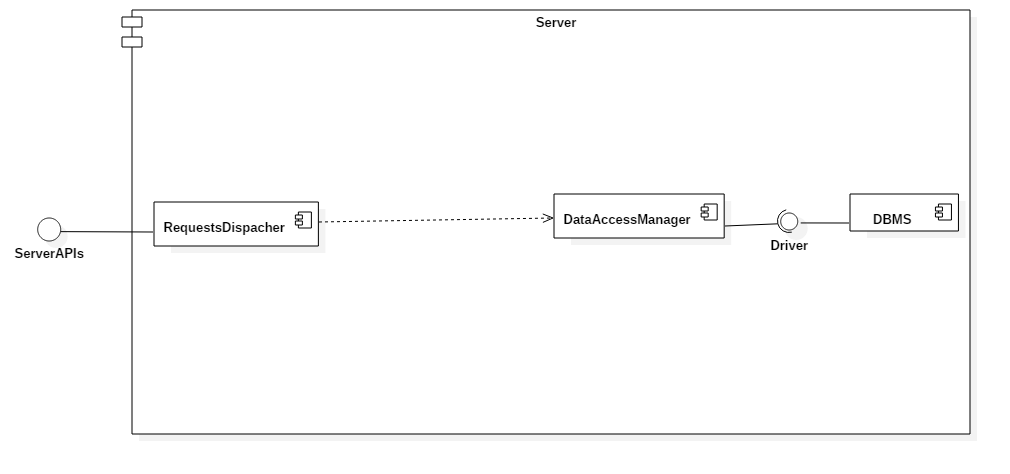
\includegraphics[scale=0.4]{images/ComponentDiagramServer}
\caption{Server Component Diagram}
\label{ref:componentdiagramserver}
\end{figure}
\begin{itemize}
\item
\textbf{RequestDispatcher:} It handles the requests from the application.
\item
\textbf{DataAccessManager:} The component that manages access to the database using a specific driver.
\item
\textbf{DBMS:} The system that will take care of the management of the data, integrated in our system using a specific driver.
\end{itemize}
